%!TEX root = ../thesis.tex
% ******************************* Thesis Appendix A ****************************

\begin{figure}[htbp!] 
\centering    
    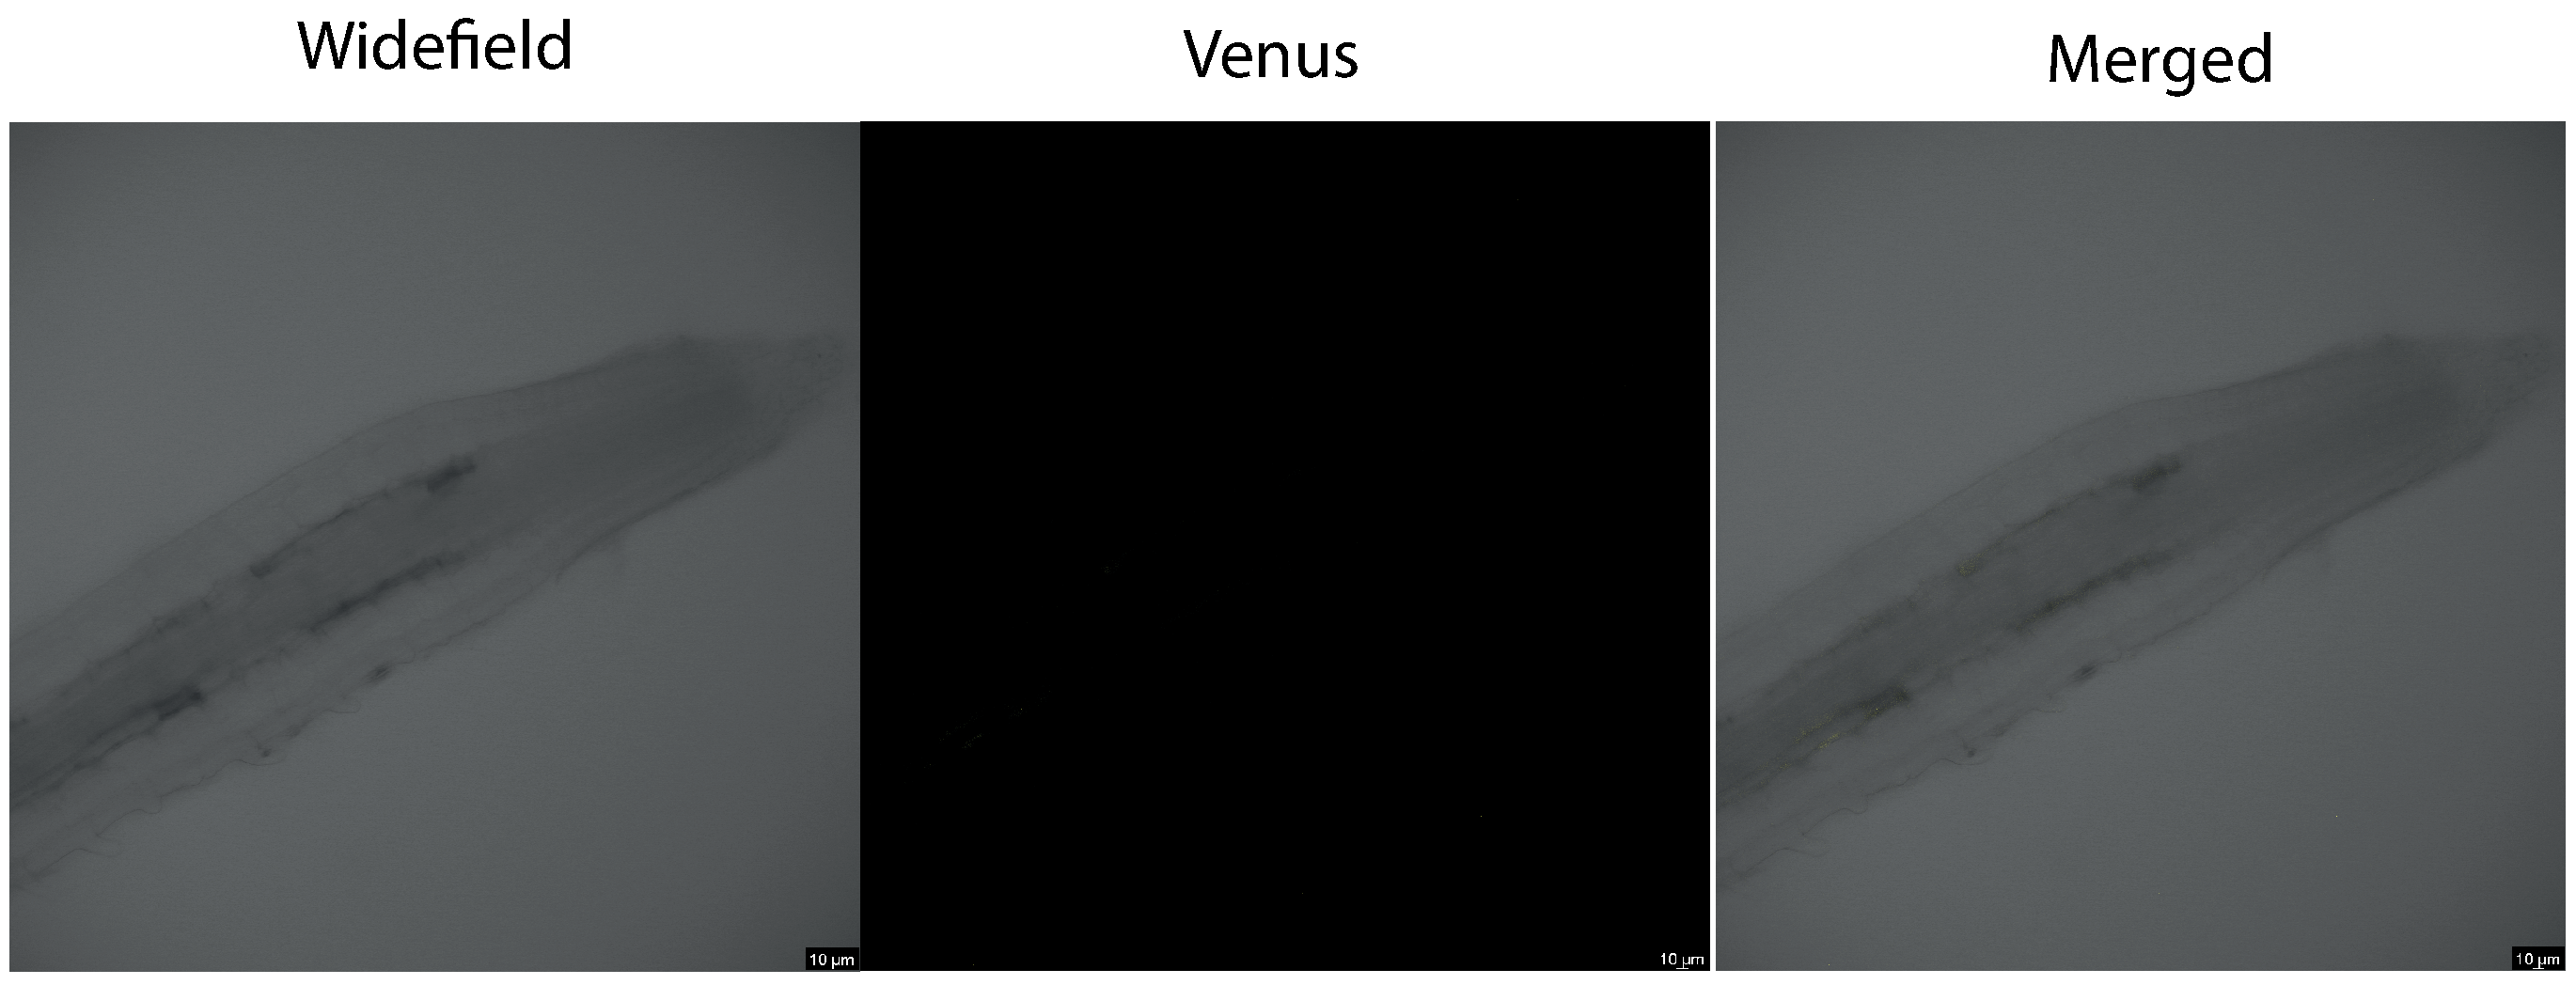
\includegraphics[width=1\textwidth]{Chapter2/Figs/Supps/FigureS1_CLSY3_Root_tip_neg.pdf}
\caption{pCLSY3::CLSY3-Venus is not expressed in the root tip}
\label{fig:clsy3_root}
\captionsetup{font=small}
    \caption*{Scale bar 10 $\mu$m.}
\end{figure}

\begin{figure}[htbp!] 
\centering    
    \includegraphics[width=1\textwidth]{Chapter2/Figs/Supps/FigureS2_CLSY1_2_Pollen.pdf}
\caption{CLSY1 and CLSY2 are not specifically expressed in the pollen}
\label{fig:clsy1_2_pollen}
\captionsetup{font=small}
    \caption*{DAPI (blue, second row) staining of pCLSY1::CLY1-eGFP (first row) and pCLSY2::CLY2-eGFP (second row) showing no expression of CLSYs (third column, GFP, green) in mature pollen. Scale bar 10 $\mu$m.}
\end{figure}

\begin{figure}[htbp!] 
\centering    
    \includegraphics[width=1\textwidth]{Chapter2/Figs/Supps/FigureS3_Pol4_Pol5_roots.pdf}
\caption{pNRPD1::NRPD1-eGFP and pNRPE1::NRPE1-eGFP are strongly expressed in the root}
\label{fig:Pol4_5_roots}
\captionsetup{font=small}
    \caption*{eGFP (green, white arrows) nuclear signal of NRPD1 (first row) and NRPE1 (second row) in the root tip of \textit{Arabidopsis}. Scale bar 10 $\mu$m.}
\end{figure}

\begin{figure}[htbp!] 
\centering    
    \includegraphics[width=1\textwidth]{Chapter2/Figs/Supps/FigureS4_Pol4_germline_no_expression.pdf}
\caption{pNRPD1 is not consistently expressed in germline tissues}
\label{fig:Pol4_germ_no_expression}
\captionsetup{font=small}
    \caption*{NRPD2 expression in microspores. eGFP (green) DAPI (blue). Scale bar 10 $\mu$m.}
\end{figure}

\begin{figure}[htbp!] 
\centering    
    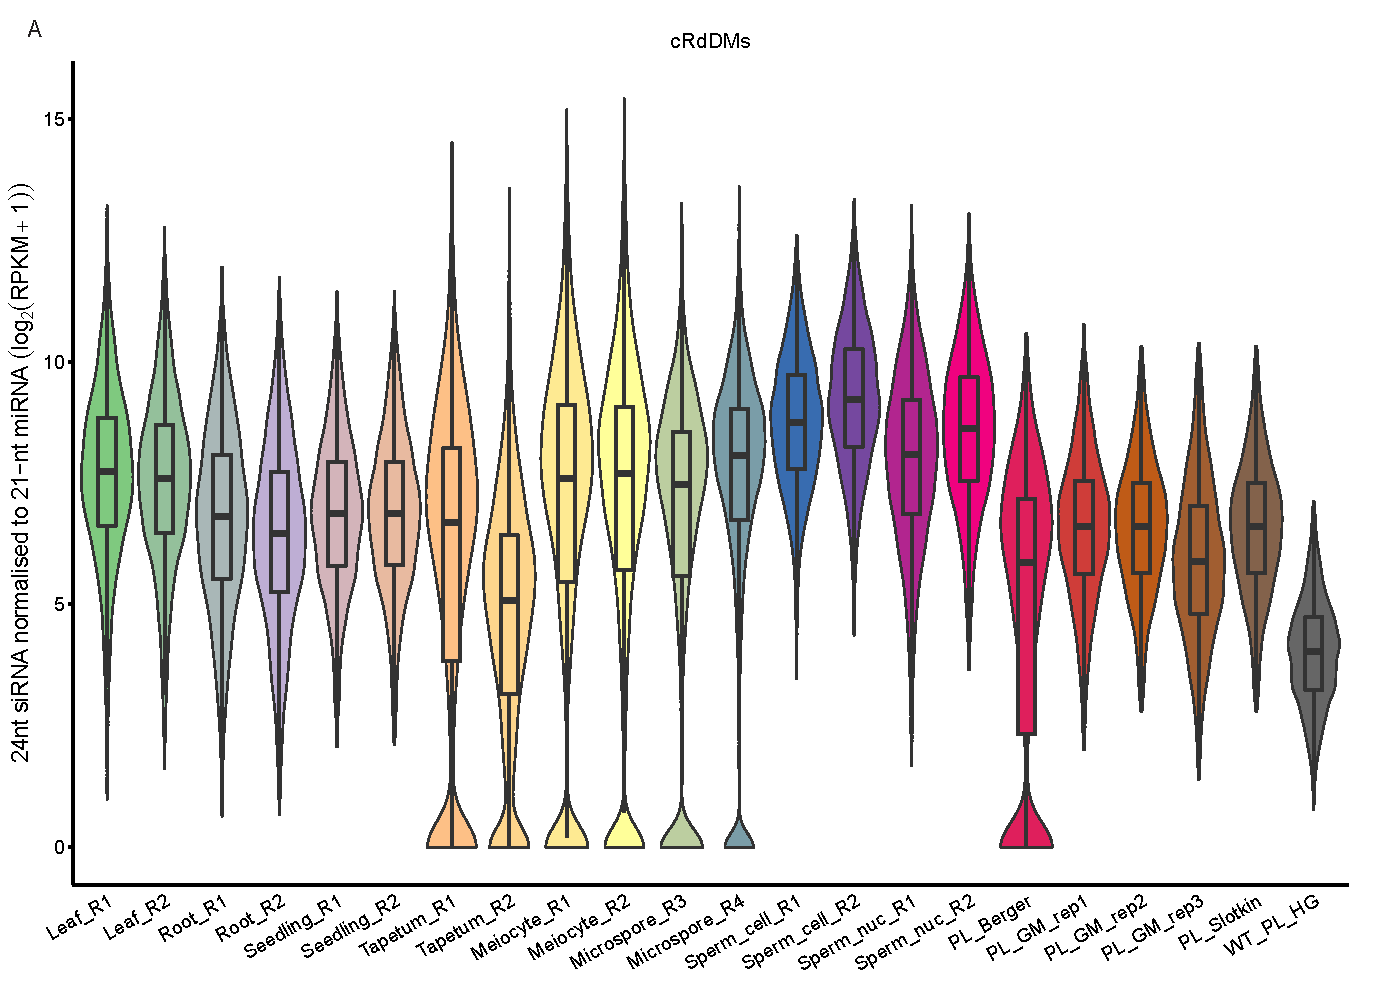
\includegraphics[width=1\textwidth]{Chapter2/Figs/Supps/FigureS7_miRNA_norm.pdf}
\caption{Violin/box plots depicting 24nt sRNA abundance normalised against total 21nt miRNAs in different somatic and germline tissues}
\label{fig:miRNA_norm}
\captionsetup{font=small}
    \caption*{}
\end{figure}

\begin{figure}[htbp!] 
\centering    
    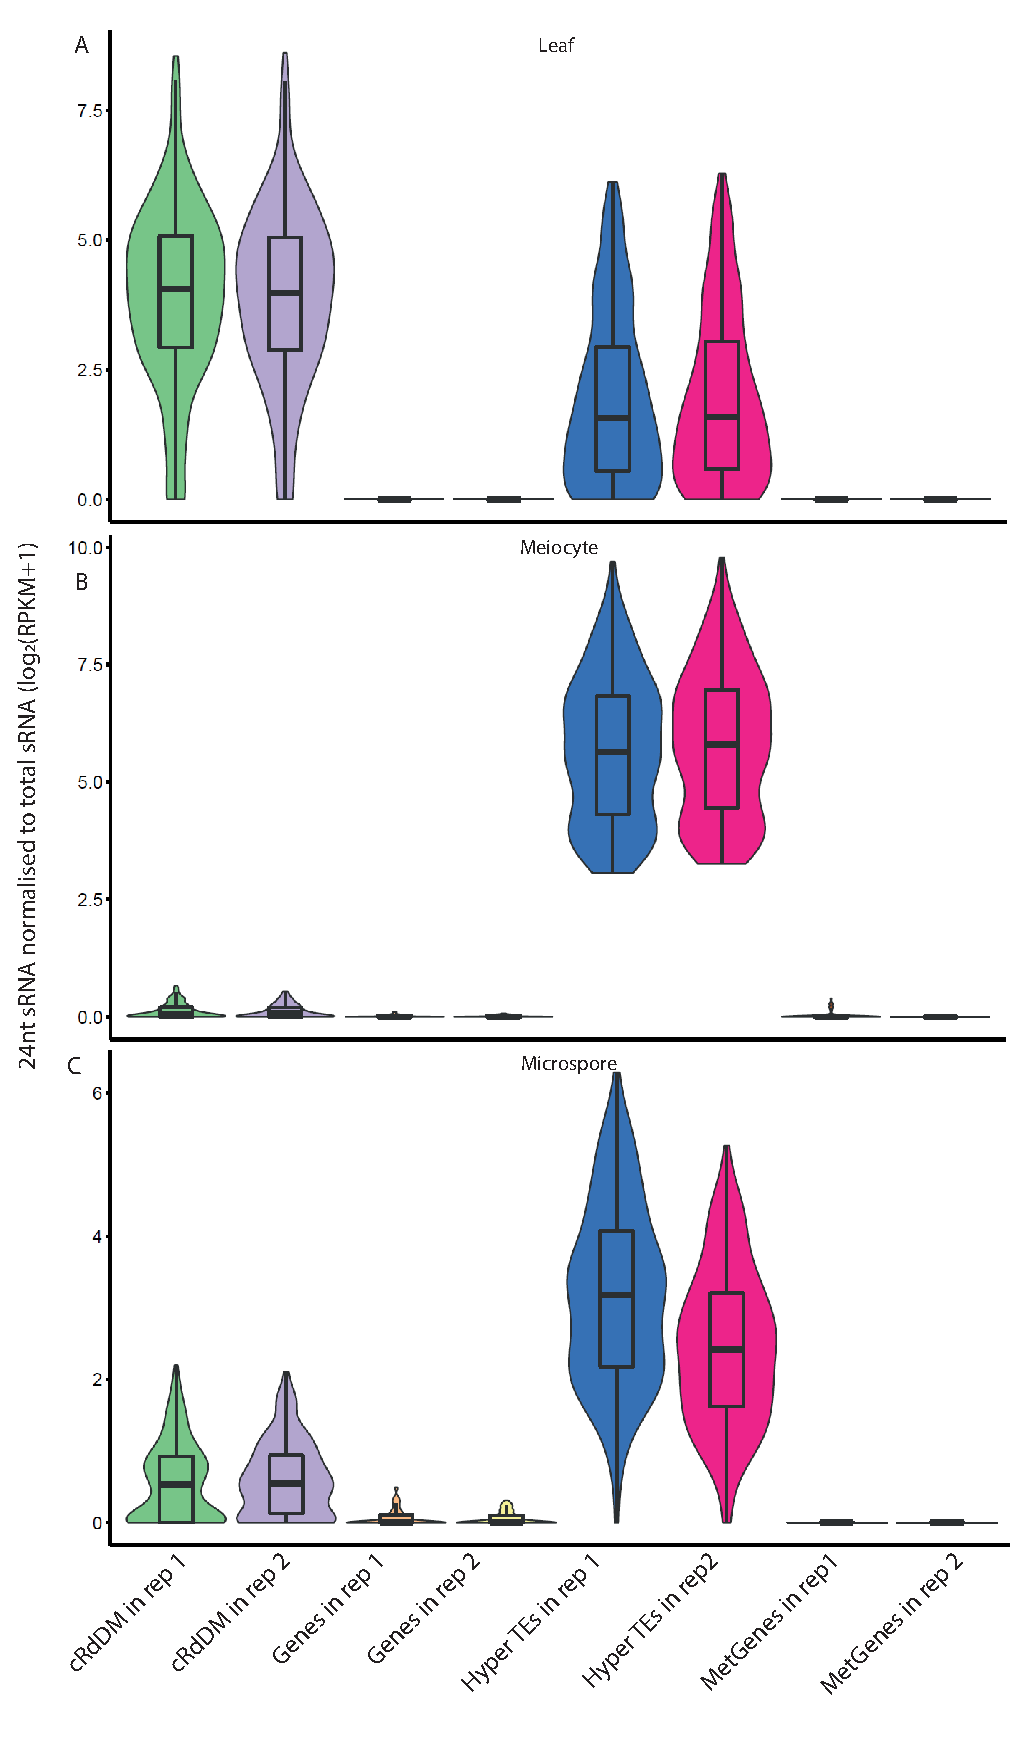
\includegraphics[width=0.8\textwidth]{Chapter2/Figs/Supps/FigureS8_boxplots_meiocyte_microspore.pdf}
\caption{Violin/box plots depicting 24nt sRNA abundance normalised against total sRNA of cRdDM, genic, HyperTE and MetGene loci in the leaf, meiocyte and microspore}
\label{fig:boxplot-MCMS}
\captionsetup{font=small}
    \caption*{}
\end{figure}

\begin{figure}[htbp!] 
\centering    
    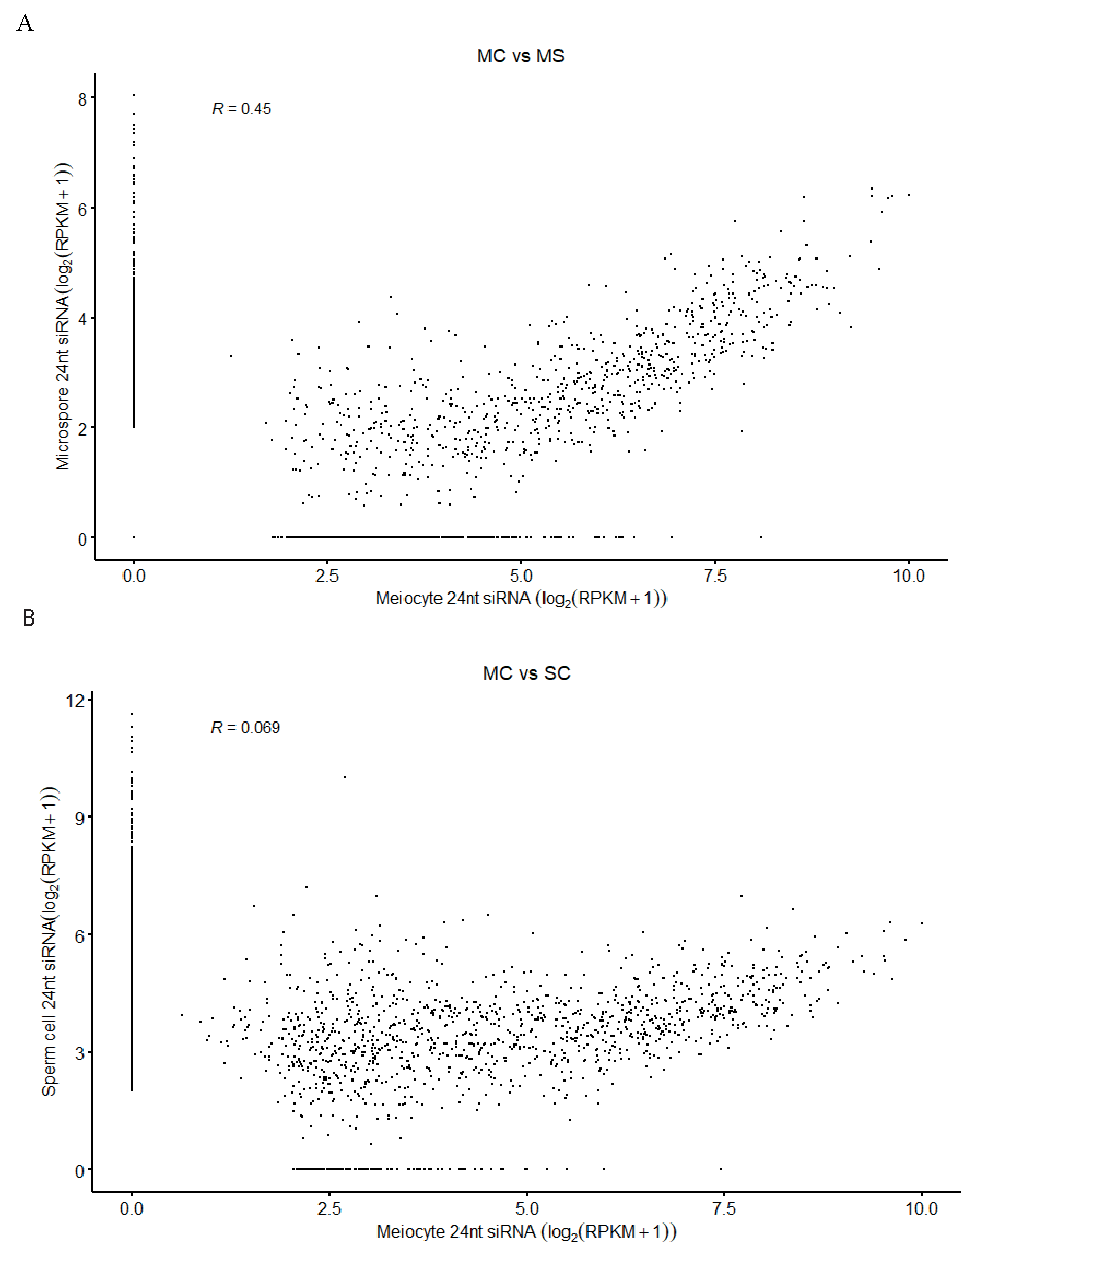
\includegraphics[width=1\textwidth]{Chapter2/Figs/Supps/FigureS5_MSSCMC_scatters.pdf}
\caption{Scatterplot comparing the abundance of 24nt sRNAs between A) the meiocyte and microspore and B) the meiocyte and the sperm cell}
\label{fig:MSSVMC_scatters}
\captionsetup{font=small}
    \caption*{}
\end{figure}

\begin{figure}[htbp!] 
\centering    
    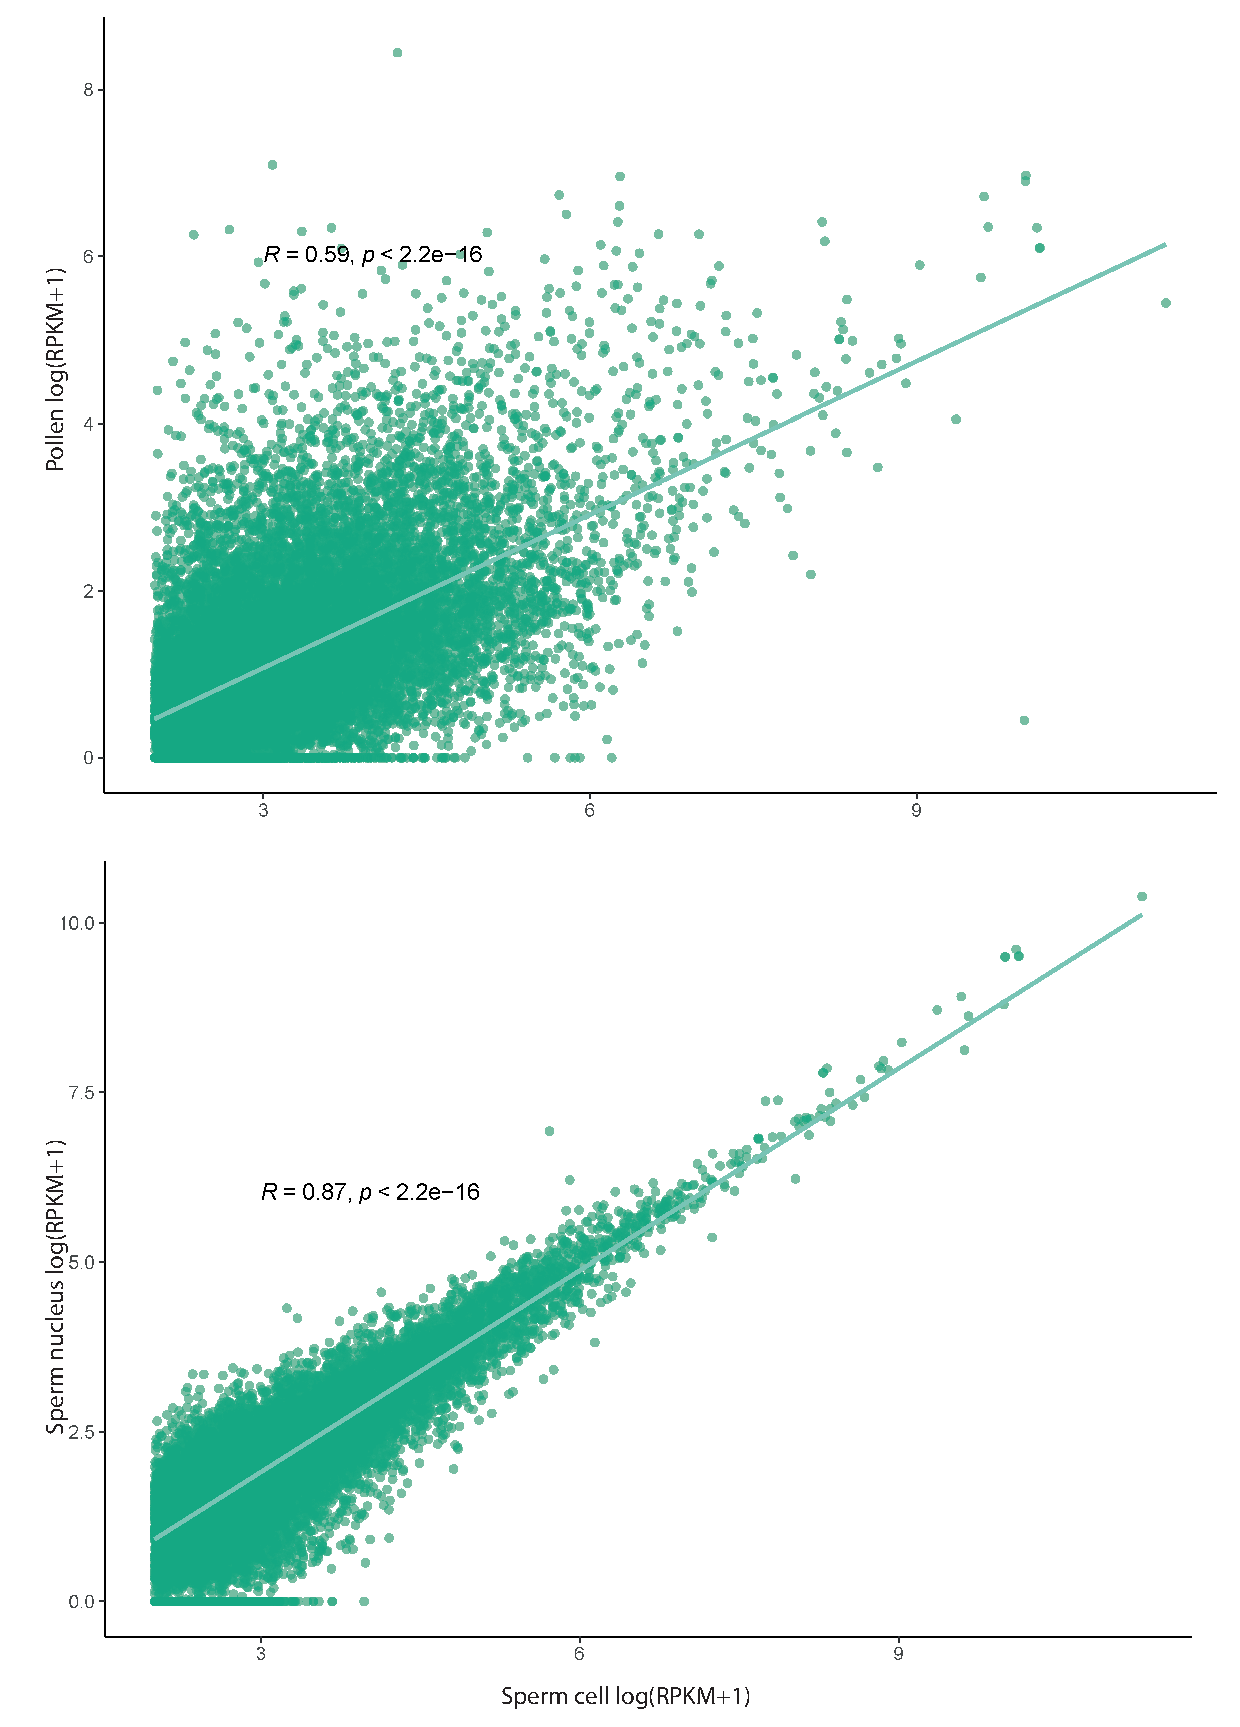
\includegraphics[width=1\textwidth]{Chapter2/Figs/Supps/PLvSC_overall.pdf}
\caption{Scatterplot comparing the abundance of 24nt sRNAs at sperm specific clusters between the pollen and the sperm cell (top graph) and the sperm nucleus and the sperm cell (bottom graph)}
\label{fig:PLvsSC_overall}
\captionsetup{font=small}
    \caption*{}
\end{figure}

\begin{figure}[htbp!] 
\centering    
    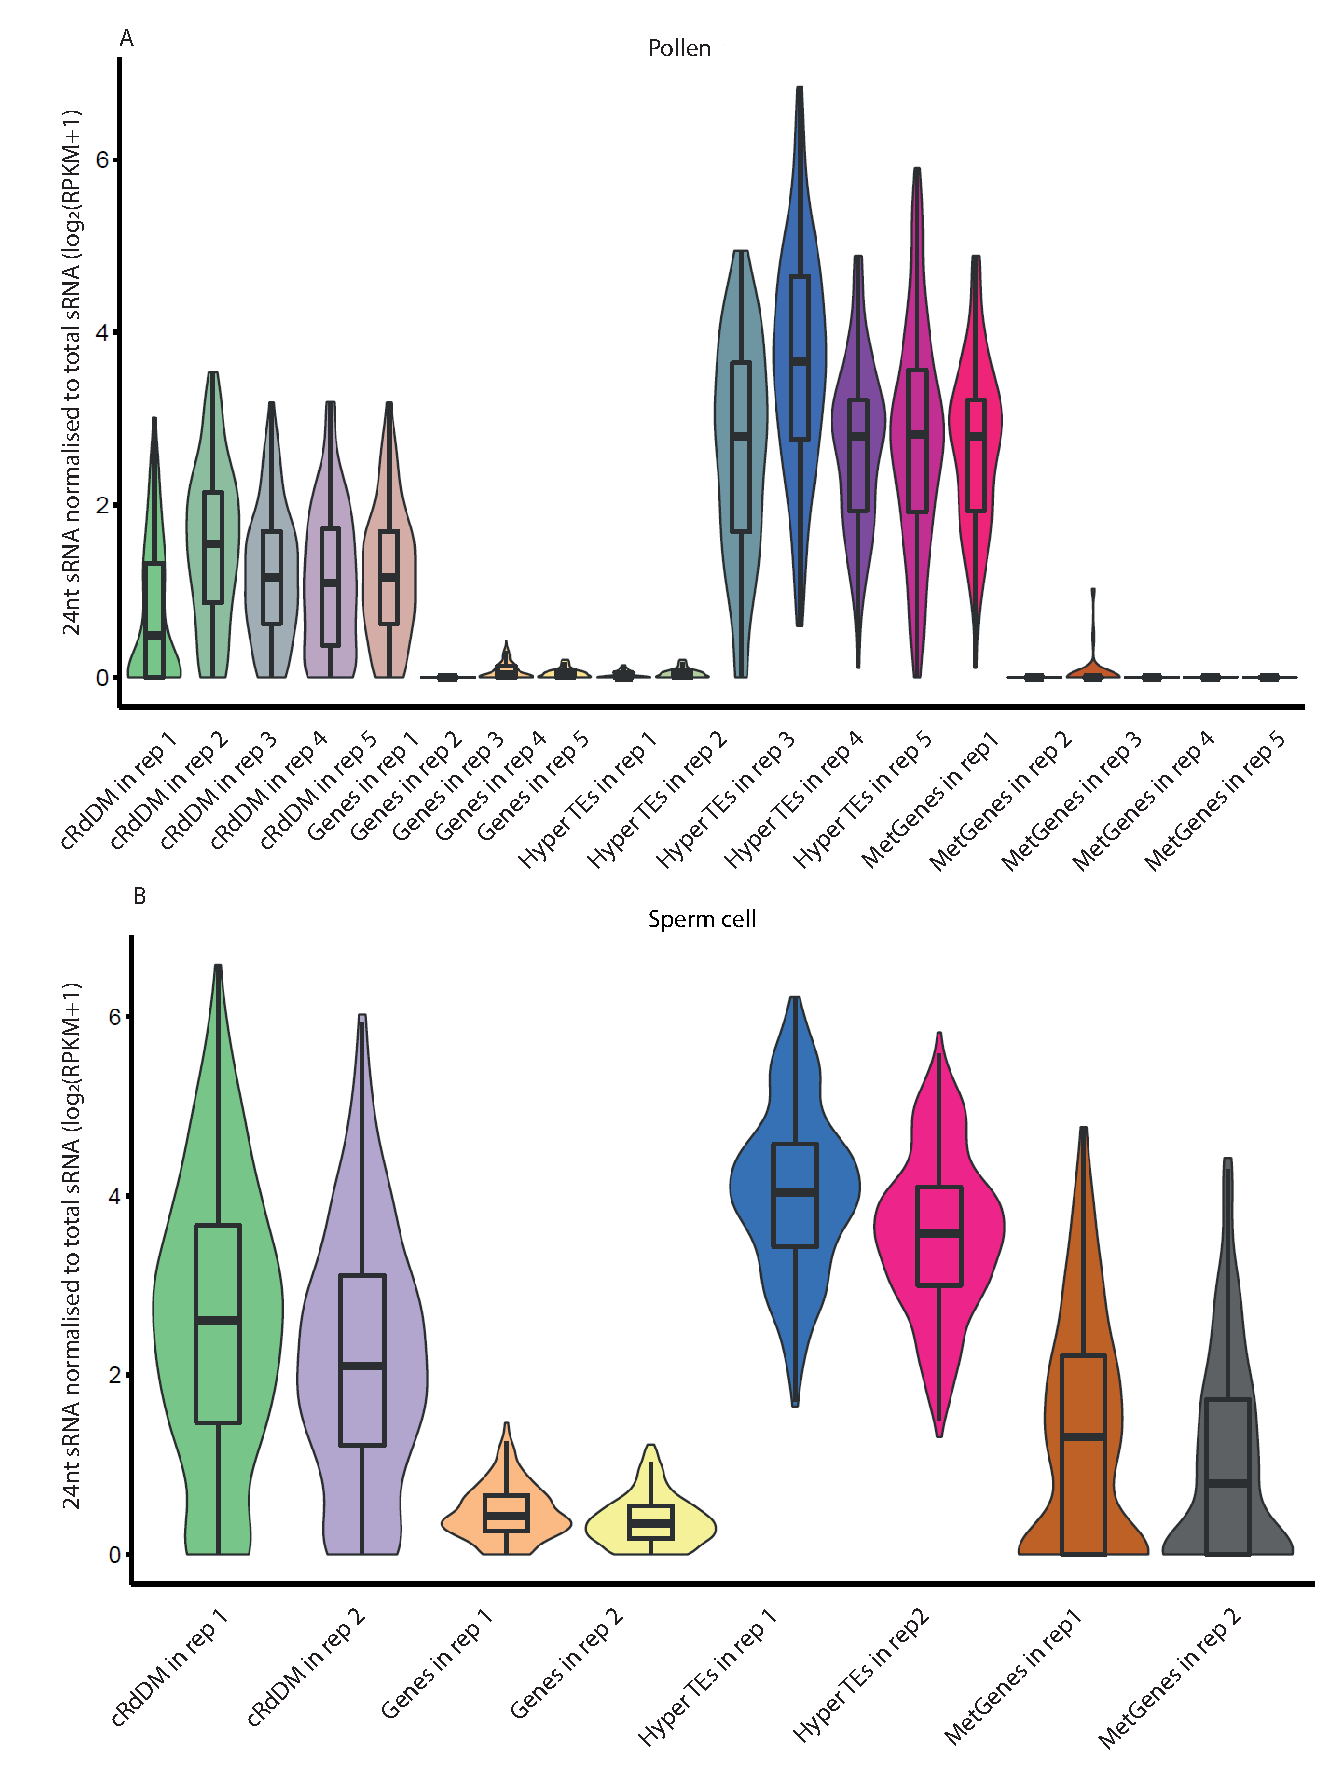
\includegraphics[width=1\textwidth]{Chapter2/Figs/Supps/FigureS9_sperm_pollen_boxplots.pdf}
\caption{Violin/box plots depicting 24nt sRNA abundance normalised against total sRNA of cRdDM, genic, HyperTE and MetGene loci in replicates of the A) pollen and B) sperm cell}
\label{fig:boxplot-SCPL}
\captionsetup{font=small}
    \caption*{}
\end{figure}

\begin{table}[htbp]
\centering
\begin{tabular}{|p{5cm}|p{3cm}|p{5cm}|}
\hline
\textbf{Line name} & & \textbf{Source} \\
\hline
pCLSY1::CLSY1-eGFP & & Feng Lab \\
pCLSY2::CLSY2-eGFP & & Feng Lab \\
pCLSY::CLSY3-Venus & &Feng Lab \\
pNRPD1::NRPD1-eGFP & & Feng Lab \\
pNRPE1::NRPE1-eGFP & & Feng Lab \\
\hline
\end{tabular}
\begin{tabular}{|p{5cm}|p{3cm}|p{5cm}|} % For 3 columns in the second part
\hline
\textbf{Library name} & \textbf{Library type} & \textbf{Source} \\
\hline
Seedling & sRNA & \cite{RN300} \\
Root & sRNA & \cite{RN301}  \\
Leaf & sRNA & \cite {RN302} \\
Tapetum & sRNA & Feng Lab \\
Meiocyte & sRNA & Feng Lab \\
Microspore & sRNA & Feng Lab (constructed by JT) \\
Sperm cell & sRNA & Feng Lab (constructed by JT) \\
Sperm nucleus & sRNA & Feng Lab (constructed by JT) \\
Pollen rep1 & sRNA & \cite{RN303}  \\
Pollen rep2 & sRNA & \cite{RN304}  \\
Pollen rep3 & sRNA & \cite{RN305}  \\
\hline
Meiocyte & BS-seq & Feng Lab \\
Microspore & BS-seq & \cite{RN306}  \\
Sperm cell & BS-seq & Feng Lab \\
Vegetative cell & BS-seq & Feng Lab \\
Seedling & BS-seq & \cite{RN307}  \\
\hline
\end{tabular}
\caption{Table depicting the line names, library types, and sources of the data presented in this chapter.}
\label{ch2:workbyothers}
\end{table}


\begin{landscape}
\small
\begin{longtable}{l|l|lll|ll|lll}
 &
  Source &
  \multicolumn{3}{c|}{Dr. James Walker} &
  \multicolumn{2}{c|}{Dr. Toby Buttress} &
  \multicolumn{3}{c}{Dr. Shaoli Zhou} \\ \hline
\endfirsthead
%
\endhead
%
Gene ID &
  Gene Name &
  Tapetum &
  Meiocyte &
  Pollen &
  Sperm &
  Vegetative &
  Meiocyte &
  Microspore &
  Sperm \\ \hline
AT3G42670 & CLSY1    & 0.069  & 2.362   & 2.425    & 0.305  & 2.407    & 1.882   & 7.154  & 1.886    \\
AT5G20420 & CLSY2    & 0.124  & 1.030   & 1.634    & 1.014  & 8.164    & 0.752   & 2.074  & 0.000    \\
AT1G05490 & CLSY3    & 11.412 & 0.534   & 0.000    & 0.039  & 0.154    & 0.439   & 1.339  & 0.000    \\
AT3G24340 & CLSY4    & 0.245  & 22.269  & 3.276    & 16.006 & 1.530    & 20.507  & 5.112  & 143.407  \\ \hline
AT2G16390 & DRD1     & 6.335  & 11.622  & 1.706    & 0.214  & 0.553    & 10.439  & 5.727  & 0.000    \\ \hline
AT1G15910 & FDM1     & 12.840 & 14.499  & 1.132    & 0.268  & 0.574    & 15.091  & 11.453 & 0.513    \\
AT4G00380 & FDM2     & 2.826  & 10.899  & 0.000    & 0.018  & 0.011    & 10.419  & 4.151  & 0.000    \\
AT3G12550 & FDM3     & 2.521  & 5.639   & 0.000    & 0.159  & 0.273    & 4.889   & 5.072  & 0.056    \\
AT1G13790 & FDM4     & 7.197  & 11.961  & 42.011   & 87.597 & 3.240    & 9.969   & 10.073 & 1306.790 \\
AT1G80780 & FDM5     & 87.837 & 20.310  & 1517.160 & 3.485  & 32.138   & 14.331  & 26.673 & 6.443    \\ \hline
AT5G15380 & DRM1     & 1.083  & 8.019   & 0.000    & 0.000  & 0.164    & 8.406   & 1.952  & 0.614    \\
AT5G14620 & DRM2     & 17.582 & 0.774   & 0.000    & 0.080  & 0.039    & 0.953   & 5.015  & 4.406    \\
AT3G17310 & DRM3     & 5.015  & 1.266   & 0.260    & 0.000  & 0.000    & 1.818   & 5.923  & 32.001   \\
AT3G22680 & RDM1     & 28.999 & 6.994   & 3.681    & 0.000  & 0.000    & 7.715   & 2.573  & 0.256    \\ \hline
AT5G04290 & KTF1     & 2.233  & 35.857  & 10.397   & 1.171  & 1.340    & 37.257  & 17.184 & 0.450    \\
AT3G49250 & KTF1 hom & 16.080 & 46.676  & 25.977   & 0.000  & 0.016    & 5.805   & 3.582  & 0.239    \\
AT2G30280 & KTF1 hom & 0.602  & 44.270  & 8.030    & 1.831  & 2.452    & 0.731   & 9.876  & 29.358   \\ \hline
AT4G36290 & MORC1    & 3.172  & 2.488   & 0.000    & 0.131  & 0.096    & 3.051   & 4.647  & 0.066    \\
AT4G36270 & MORC2    & 0.485  & 16.507  & 0.000    & 0.000  & 2438.620 & 10.101  & 1.316  & 3.145    \\
AT4G36270 & MORC3    & 0.097  & 16.216  & 0.000    & 0.017  & 0.000    & 11.087  & 3.810  & 1.964    \\
AT5G50780 & MORC4    & 0.679  & 52.595  & 17.862   & 35.680 & 1.265    & 53.671  & 9.817  & 495.904  \\
AT5G13130 & MORC5    & 0.000  & 3.191   & 0.261    & 0.053  & 0.046    & 3.169   & 19.304 & 0.218    \\
AT1G19100 & MORC6    & 4.610  & 22.521  & 8.392    & 0.000  & 50.949   & 23.561  & 5.809  & 0.000    \\
AT4G24970 & MORC7    & 0.051  & 0.251   & 0.806    & 0.017  & 0.253    & 0.335   & 3.584  & 0.756    \\ \hline
AT5G04940 & SUVH1    & 3.269  & 4.217   & 0.000    & 0.281  & 0.159    & 4.097   & 6.219  & 0.708    \\
AT2G33290 & SUVH2    & 1.546  & 9.811   & 0.369    & 0.314  & 0.659    & 13.030  & 1.673  & 2.822    \\
AT1G73100 & SUVH3    & 3.373  & 0.659   & 3.395    & 1.077  & 0.491    & 0.526   & 4.473  & 10.688   \\
AT5G13960 & SUVH4    & 5.464  & 8.346   & 1.073    & 4.163  & 0.355    & 3.007   & 6.048  & 32.060   \\
AT2G35160 & SUVH5    & 8.072  & 24.464  & 7.386    & 16.224 & 2.036    & 21.982  & 17.397 & 250.727  \\
AT2G22740 & SUVH6    & 3.692  & 22.468  & 97.319   & 20.015 & 52.259   & 23.143  & 6.751  & 34.313   \\
AT1G17770 & SUVH7    & 0.000  & 0.318   & 0.838    & 0.320  & 0.168    & 0.295   & 0.000  & 6.145    \\
AT2G24740 & SUVH8    & 0.000  & 1.004   & 0.000    & 0.000  & 0.022    & 0.848   & 1.833  & 0.000    \\
AT4G13460 & SUVH9    & 4.288  & 1.660   & 5.555    & 0.960  & 0.996    & 1.520   & 3.572  & 1.321    \\
AT2G05900 & SUVH10   & 0.000  & 0.000   & 0.000    & 0.000  & 0.169    & 0.000   & 0.000  & 0.000    \\
AT5G47150 & SUVH hom & 0.911  & 3.590   & 0.000    & 0.000  & 0.000    & 4.070   & 0.856  & 0.000    \\
AT5G47160 & SUVH hom & 0.006  & 4.307   & 0.000    & 3.233  & 0.000    & 3.451   & 1.243  & 25.517   \\ \hline
AT1G04050 & SUVR1    & 30.801 & 20.204  & 13.628   & 7.794  & 0.156    & 3.913   & 7.442  & 46.306   \\
AT5G43990 & SUVR2    & 4.326  & 22.124  & 0.000    & 0.022  & 0.028    & 20.202  & 8.224  & 0.000    \\
AT3G03750 & SUVR3    & 9.598  & 1.024   & 7.831    & 1.528  & 1.647    & 1.600   & 4.982  & 3.445    \\
AT3G04380 & SUVR4    & 0.935  & 14.174  & 0.000    & 0.858  & 0.053    & 11.715  & 6.492  & 12.778   \\
AT2G23740 & SUVR5    & 4.494  & 1.785   & 4.050    & 1.021  & 3.892    & 1.802   & 20.790 & 0.178    \\ \hline
AT4G08350 & DMS3     & 18.867 & 6.984   & 0.000    & 4.929  & 8.594    & 59.555  & 23.154 & 39.541   \\
AT2G34210 & DMS4     & 15.176 & 0.640   & 0.000    & 1.831  & 2.452    & 0.731   & 9.876  & 29.358   \\ \hline
AT4G35800 & NRPB1    & 9.760  & 124.307 & 53.801   & 16.013 & 24.952   & 179.741 & 54.232 & 22.260   \\
AT5G09920 & NRPB4    & 33.043 & 3.486   & 10.789   & 2.164  & 0.803    & 3.303   & 23.280 & 154.460  \\
AT3G22320 & NRPB5A   & 44.975 & 5.953   & 5.603    & 3.139  & 0.925    & 4.689   & 26.076 & 23.576   \\
AT5G57980 & NRPB5L1  & 0.727  & 0.721   & 6.832    & 0.000  & 1134.040 & 0.511   & 12.250 & 0.000    \\
AT5G45140 & NRPC2    & 1.005  & 41.613  & 1.371    & 0.357  & 0.129    & 44.598  & 20.155 & 4.112    \\
AT1G63020 & NRPD1    & 0.000  & 0.769   & 0.000    & 0.558  & 0.016    & 0.880   & 5.191  & 1.894    \\
AT3G23780 &
  \begin{tabular}[c]{@{}l@{}}NRPD2/\\ NRPE2\end{tabular} &
  14.986 &
  52.199 &
  0.247 &
  0.200 &
  0.063 &
  62.401 &
  13.488 &
  0.000 \\
AT3G18090 & NRPD2B   & 0.033  & 4.055   & 0.000    & 0.006  & 0.005    & 5.035   & 1.692  & 0.000    \\
AT4G15950 & NRPD4    & 19.473 & 1.273   & 0.000    & 0.478  & 0.567    & 0.552   & 4.757  & 3.143    \\
AT2G41340 & NRPD5B   & 0.000  & 0.046   & 0.000    & 0.000  & 0.000    & 0.072   & 0.000  & 0.000    \\
AT2G40030 & NRPE1    & 1.082  & 24.894  & 0.000    & 0.000  & 0.000    & 24.162  & 8.895  & 0.000    \\
AT3G57070 & NRPE5A   & 29.421 & 0.216   & 5.750    & 0.000  & 0.000    & 0.113   & 5.075  & 0.000    \\
AT3G54490 & NRPE5C   & 17.226 & 4.276   & 0.000    & 0.000  & 0.000    & 2.725   & 11.066 & 0.000    \\
AT3G16980 & NRPE9A   & 6.392  & 1.796   & 0.000    & 0.135  & 0.610    & 2.602   & 3.470  & 6.034    \\
AT4G16265 & NRPE9B   & 0.379  & 2.491   & 0.000    & 0.000  & 0.000    & 1.092   & 6.801  & 0.000    \\
AT4G21710 & NRPPB2   & 12.819 & 48.481  & 7.926    & 3.972  & 6.622    & 49.733  & 23.705 & 0.608    \\ \hline
AT1G48405 & AGO1     & 92.316 & 62.973  & 0.320    & 0.399  & 0.752    & 84.635  & 45.999 & 0.721    \\
AT1G31280 & AGO2     & 1.897  & 3.440   & 0.243    & 0.099  & 0.296    & 4.270   & 8.758  & 0.000    \\
AT1G31290 & AGO3     & 0.000  & 0.040   & 0.000    & 0.047  & 1.069    & 0.023   & 0.138  & 0.038    \\
AT2G27040 & AGO4     & 4.670  & 13.424  & 0.315    & 0.127  & 0.070    & 13.311  & 62.406 & 0.000    \\
AT2G27880 & AGO5     & 29.327 & 23.341  & 5.436    & 0.000  & 527.075  & 26.161  & 11.675 & 41.270   \\
AT2G32940 & AGO6     & 0.271  & 9.677   & 0.481    & 0.567  & 0.014    & 9.734   & 3.238  & 2.067    \\
AT1G69440 & AGO7     & 0.000  & 0.821   & 0.000    & 0.113  & 0.432    & 0.659   & 0.693  & 0.000    \\
AT5G21030 & AGO8     & 0.000  & 0.011   & 0.000    & 4.486  & 15.940   & 0.016   & 0.000  & 0.601    \\
AT5G21150 & AGO9     & 53.737 & 110.374 & 49.874   & 75.117 & 1.354    & 128.692 & 28.993 & 739.026  \\
AT5G43810 & AGO10    & 3.353  & 2.119   & 0.991    & 0.467  & 0.034    & 2.410   & 2.815  & 0.575    \\ \hline
AT1G01040 & DCL1     & 5.333  & 1.900   & 2.926    & 3.523  & 1.612    & 1.612   & 17.886 & 17.858   \\
AT3G03300 & DCL2     & 7.214  & 15.916  & 1.286    & 0.171  & 0.353    & 5.327   & 14.302 & 0.000    \\
AT3G43920 & DCL3     & 6.432  & 2.550   & 0.000    & 0.066  & 0.719    & 2.545   & 15.484 & 3.168    \\
AT5G20320 & DCL4     & 2.318  & 26.588  & 0.000    & 0.013  & 0.107    & 28.061  & 2.743  & 0.071    \\ \hline
AT4G11130 & RDR2     & 0.368  & 3.019   & 0.946    & 0.399  & 0.599    & 2.796   & 2.608  & 11.298   \\
AT3G49500 & RDR6     & 3.296  & 18.003  & 0.000    & 0.131  & 0.048    & 18.123  & 6.580  & 0.000    \\ \hline
AT5G23570 & SGS3     & 8.552  & 73.316  & 0.000    & 0.100  & 0.160    & 83.520  & 13.197 & 1.387  \\
\caption{FPKM values of RdDM components in germline tissues (data from Dr. James Walker, Dr Shaoli Zhou and Dr. Toby Buttress)}\\
\label{tab:FPKM_germ}\\
\end{longtable}
\end{landscape}

\begin{landscape}
\begin{longtable}{l|l|llll|lll}
          & Source                                                 & \multicolumn{4}{c|}{Dr. James Walker}   & \multicolumn{3}{c}{Dr. Shaoli Zhou} \\ \hline
\endfirsthead
%
\endhead
%
Gene ID   & Gene name                                              & Seedling & Rosette & Columella & Embryo & Seedling    & Leaf      & Root      \\ \hline
AT3G42670 & CLSY1    & 0.961  & 1.208  & 13.150 & 2.733   & 1.659  & 1.316  & 1.733  \\
AT5G20420 & CLSY2    & 0.079  & 0.061  & 1.083  & 0.000   & 0.165  & 0.000  & 0.120  \\
AT1G05490 & CLSY3    & 0.092  & 0.022  & 0.027  & 20.036  & 0.057  & 0.037  & 0.203  \\
AT3G24340 & CLSY4    & 0.109  & 0.040  & 0.126  & 0.256   & 0.216  & 0.150  & 0.209  \\ \hline
AT2G16390 & DRD1     & 1.626  & 2.243  & 2.916  & 1.204   & 2.263  & 3.352  & 1.793  \\ \hline
AT1G15910 & FDM1     & 5.530  & 4.794  & 6.337  & 15.276  & 5.959  & 7.078  & 5.874  \\
AT4G00380 & FDM2     & 1.134  & 0.716  & 1.026  & 9.490   & 2.840  & 1.409  & 0.595  \\
AT3G12550 & FDM3     & 2.176  & 2.500  & 3.021  & 1.139   & 1.355  & 4.527  & 2.760  \\
AT1G13790 & FDM4     & 0.894  & 0.887  & 1.007  & 0.124   & 0.832  & 2.610  & 0.254  \\
AT1G80780 & FDM5     & 54.647 & 67.899 & 62.413 & 107.629 & 8.427  & 25.398 & 14.350 \\ \hline
AT5G15380 & DRM1     & 0.019  & 0.019  & 0.004  & 4.552   & 0.000  & 0.016  & 0.033  \\
AT5G14620 & DRM2     & 2.704  & 3.862  & 5.379  & 4.888   & 4.719  & 2.662  & 3.300  \\
AT3G17310 & DRM3     & 4.623  & 5.665  & 5.569  & 3.255   & 7.510  & 6.246  & 4.070  \\ \hline
AT3G22680 & RDM1     & 17.900 & 14.269 & 22.518 & 366.562 & 11.155 & 4.951  & 16.888 \\ \hline
AT5G04290 & KTF1     & 3.203  & 3.124  & 3.715  & 7.349   & 6.860  & 15.337 & 5.311  \\
AT3G49250 & KTF1 hom & 9.321  & 11.530 & 17.212 & 25.813  & 2.319  & 2.388  & 2.370  \\
AT2G30280 & KTF1 hom & 0.214  & 0.082  & 0.053  & 0.120   & 4.624  & 7.242  & 5.133  \\ \hline
AT4G36290 & MORC1    & 3.733  & 4.219  & 5.787  & 2.180   & 3.048  & 8.723  & 5.013  \\
AT4G36270 & MORC2    & 1.298  & 6.368  & 1.383  & 0.032   & 0.965  & 3.306  & 0.057  \\
AT4G36270 & MORC3    & 0.645  & 0.924  & 0.780  & 0.000   & 0.068  & 0.829  & 0.738  \\
AT5G50780 & MORC4    & 2.468  & 2.601  & 2.204  & 3.015   & 2.191  & 6.396  & 4.145  \\
AT5G13130 & MORC5    & 0.017  & 0.161  & 0.000  & 0.060   & 0.307  & 0.263  & 0.047  \\
AT1G19100 & MORC6    & 2.030  & 2.228  & 5.795  & 0.409   & 2.092  & 2.747  & 2.192  \\
AT4G24970 & MORC7    & 1.223  & 3.298  & 2.819  & 0.000   & 1.512  & 4.043  & 1.315  \\ \hline
AT5G04940 & SUVH1    & 3.438  & 2.470  & 4.917  & 6.052   & 3.990  & 4.242  & 4.225  \\
AT2G33290 & SUVH2    & 2.245  & 2.998  & 1.156  & 5.306   & 4.415  & 4.289  & 2.697  \\
AT1G73100 & SUVH3    & 3.982  & 3.510  & 11.081 & 13.420  & 6.664  & 6.552  & 4.452  \\
AT5G13960 & SUVH4    & 2.410  & 2.030  & 3.627  & 47.075  & 3.758  & 1.401  & 5.955  \\
AT2G35160 & SUVH5    & 0.910  & 0.324  & 0.894  & 4.801   & 0.545  & 0.406  & 1.354  \\
AT2G22740 & SUVH6    & 2.887  & 4.517  & 5.086  & 2.496   & 4.822  & 7.003  & 4.470  \\
AT1G17770 & SUVH7    & 0.000  & 0.000  & 0.000  & 0.000   & 0.000  & 0.000  & 0.000  \\
AT2G24740 & SUVH8    & 0.015  & 0.000  & 0.007  & 0.558   & 0.000  & 0.000  & 0.027  \\
AT4G13460 & SUVH9    & 7.398  & 8.519  & 6.302  & 4.992   & 7.239  & 11.555 & 7.267  \\
AT2G05900 & SUVH10   & 0.000  & 0.000  & 0.000  & 0.000   & 0.103  & 0.000  & 0.000  \\
AT5G47150 & SUVH hom & 0.033  & 0.022  & 0.000  & 0.000   & 0.065  & 0.000  & 0.188  \\
AT5G47160 & SUVH hom & 0.354  & 0.131  & 1.544  & 0.000   & 0.293  & 0.105  & 0.695  \\ \hline
AT1G04050 & SUVR1    & 18.759 & 6.641  & 11.463 & 631.832 & 0.603  & 0.632  & 1.471  \\
AT5G43990 & SUVR2    & 1.374  & 1.293  & 3.316  & 4.269   & 1.004  & 1.233  & 2.264  \\
AT3G03750 & SUVR3    & 4.171  & 5.450  & 6.394  & 51.586  & 6.049  & 3.844  & 4.321  \\
AT3G04380 & SUVR4    & 1.302  & 1.193  & 2.034  & 1.404   & 0.791  & 2.723  & 1.687  \\
AT2G23740 & SUVR5    & 2.568  & 2.736  & 15.758 & 0.041   & 2.324  & 5.222  & 3.804  \\ \hline
AT4G08350 & DMS3     & 2.643  & 2.858  & 4.623  & 12.359  & 11.099 & 18.797 & 18.205 \\
AT2G34210 & DMS4     & 4.667  & 4.279  & 2.068  & 6.444   & 4.624  & 7.242  & 5.133  \\ \hline
AT4G35800 & NRPB1    & 8.264  & 11.717 & 27.087 & 4.111   & 15.824 & 42.750 & 16.185 \\
AT5G09920 & NRPB4    & 34.759 & 36.097 & 52.051 & 71.478  & 29.417 & 22.003 & 26.689 \\
AT3G22320 & NRPB5A                                                 & 36.980   & 38.321  & 45.945    & 36.660 & 48.069      & 26.584    & 40.246    \\
AT5G57980 & NRPB5L1  & 4.188  & 0.049  & 4.656  & 0.000   & 0.662  & 0.000  & 10.906 \\
AT5G45140 & NRPC2    & 3.125  & 2.325  & 3.281  & 1.950   & 2.685  & 4.914  & 5.913  \\
AT1G63020 & NRPD1    & 0.542  & 0.847  & 7.558  & 0.337   & 0.915  & 1.334  & 0.975  \\
AT3G23780 & \begin{tabular}[c]{@{}l@{}}NRPD2/\\ NRPE2\end{tabular} & 2.514    & 3.646   & 8.900     & 21.602 & 4.794       & 6.592     & 4.763     \\
AT3G18090 & NRPD2B   & 1.075  & 0.643  & 0.740  & 0.931   & 0.470  & 1.057  & 0.715  \\
AT4G15950 & NRPD4    & 6.346  & 8.052  & 8.840  & 3.641   & 7.663  & 5.590  & 4.387  \\
AT2G41340 & NRPD5B   & 3.469  & 0.685  & 0.045  & 0.000   & 3.643  & 0.053  & 0.328  \\
AT2G40030 & NRPE1    & 0.820  & 0.753  & 2.561  & 9.645   & 0.914  & 1.668  & 0.818  \\
AT3G57070 & NRPE5A   & 19.086 & 24.535 & 20.167 & 18.248  & 17.301 & 4.845  & 18.518 \\
AT3G54490 & NRPE5C   & 0.056  & 0.256  & 0.352  & 7.184   & 0.000  & 0.000  & 0.000  \\
AT3G16980 & NRPE9A   & 1.164  & 0.689  & 3.998  & 35.167  & 1.109  & 1.156  & 1.084  \\
AT4G16265 & NRPE9B   & 14.513 & 10.429 & 5.805  & 130.605 & 7.653  & 2.782  & 13.837 \\
AT4G21710 & NRPPB2   & 7.853  & 9.516  & 21.464 & 7.309   & 8.877  & 13.461 & 15.022 \\ \hline
AT1G48405 & AGO1     & 18.825 & 22.312 & 46.941 & 94.760  & 20.245 & 19.846 & 42.322 \\
AT1G31280 & AGO2     & 3.051  & 2.911  & 8.118  & 45.176  & 2.932  & 4.019  & 5.520  \\
AT1G31290 & AGO3     & 0.564  & 0.105  & 0.185  & 0.582   & 1.101  & 0.273  & 0.033  \\
AT2G27040 & AGO4     & 5.175  & 5.423  & 11.535 & 118.524 & 5.237  & 7.882  & 8.325  \\
AT2G27880 & AGO5     & 0.023  & 0.000  & 0.000  & 43.974  & 0.019  & 0.018  & 0.019  \\
AT2G32940 & AGO6     & 0.469  & 0.514  & 0.775  & 1.389   & 0.322  & 0.203  & 0.658  \\
AT1G69440 & AGO7     & 0.886  & 1.762  & 0.479  & 2.809   & 1.853  & 3.459  & 0.849  \\
AT5G21030 & AGO8     & 0.015  & 0.042  & 0.181  & 0.000   & 0.000  & 0.000  & 0.023  \\
AT5G21150 & AGO9     & 0.105  & 0.023  & 0.022  & 231.763 & 0.068  & 0.370  & 0.000  \\
AT5G43810 & AGO10    & 5.387  & 4.099  & 4.786  & 24.060  & 5.745  & 10.163 & 4.985  \\ \hline
AT1G01040 & DCL1     & 9.284  & 12.103 & 4.714  & 0.287   & 1.368  & 9.010  & 3.317  \\
AT3G03300 & DCL2     & 6.672  & 7.583  & 9.472  & 1.559   & 1.049  & 3.269  & 3.074  \\
AT3G43920 & DCL3     & 0.745  & 1.353  & 2.398  & 0.385   & 0.680  & 1.969  & 0.864  \\
AT5G20320 & DCL4     & 1.892  & 3.328  & 4.931  & 0.435   & 1.517  & 3.871  & 2.199  \\ \hline
AT4G11130 & RDR2     & 0.842  & 0.976  & 10.446 & 0.446   & 1.477  & 1.104  & 1.943  \\
AT3G49500 & RDR6     & 6.338  & 8.269  & 6.807  & 65.028  & 6.535  & 7.052  & 5.326  \\ \hline
AT5G23570 & SGS3     & 3.240  & 2.973  & 6.134  & 4.181   & 3.217  & 9.856  & 4.575 \\ 
\caption{FPKM levels of somatic RdDM components (data from Dr. James Walker, Dr Shaoli Zhou and Dr. Toby Buttress)} \\
\label{tab:FPKM_soma}\\
\end{longtable}
\end{landscape}

\begin{landscape}
\begin{longtable}{ll|llllllll|ll}
Gene name & Gene ID & Tapetum & Meiocyte & Microspore & Sperm rep1 & Sperm rep2 & Vegetative & Pollen & Embryo & Seedling & Leaf \\ \hline
\endfirsthead
%
\endhead
%
VIM4 & AT1G66040 & 0.000  & 0.208  & 0.278  & 129.821 & 4.492  & 0.341    & 9.202  & 0.328  & 0.011 & 0.000 \\
VIM2 & AT1G66050 & 0.099  & 2.658  & 7.049  & 35.078  & 0.622  & 0.055    & 1.011  & 5.699  & 0.290 & 0.393 \\
VIM1 & AT1G57820 & 14.205 & 38.148 & 9.812  & 317.158 & 0.000  & 1320.830 & 4.708  & 67.593 & 6.529 & 3.569 \\
VIM3 & AT5G39550 & 3.176  & 41.704 & 23.178 & 188.381 & 21.844 & 0.510    & 11.350 & 20.306 & 5.242 & 1.057 \\
VIM5 & AT1G57800 & 0.000  & 0.037  & 1.877  & 63.004  & 4.596  & 0.300    & 2.614  & 0.697  & 0.005 & 0.000 \\
\caption{VIM FPKM expression in soma and germline (data from Dr. James Walker, Dr Shaoli Zhou and Dr. Toby Buttress)} \\
\label{tab:VIM_expression}\\
\end{longtable}
\end{landscape}